%%%%%%%%%%%%%%%%%%%%%%%%%%%%%%%%%%%%%%%%%
% Structured General Purpose Assignment
% LaTeX Template
%
% This template has been downloaded from:
% http://www.latextemplates.com
%
% Original author:
% Ted Pavlic (http://www.tedpavlic.com)
%
% Note:
% The \lipsum[#] commands throughout this template generate dummy text
% to fill the template out. These commands should all be removed when
% writing assignment content.
%
%%%%%%%%%%%%%%%%%%%%%%%%%%%%%%%%%%%%%%%%%

%----------------------------------------------------------------------------------------
%	PACKAGES AND OTHER DOCUMENT CONFIGURATIONS
%----------------------------------------------------------------------------------------

\documentclass{article}

\usepackage{multirow}
\usepackage{amssymb}
\usepackage[fleqn]{amsmath}
\usepackage{url}

\usepackage{fancyhdr} % Required for custom headers
\usepackage{lastpage} % Required to determine the last page for the footer
\usepackage{extramarks} % Required for headers and footers
\usepackage{graphicx} % Required to insert images
\usepackage{lipsum} % Used for inserting dummy 'Lorem ipsum' text into the template

% Margins
\topmargin=-0.45in
\evensidemargin=0in
\oddsidemargin=0in
\textwidth=6.5in
\textheight=9.0in
\headsep=0.25in

\linespread{1.1} % Line spacing

% Set up the header and footer
\pagestyle{fancy}
\lhead{\hmwkAuthorName} % Top left header
\chead{\hmwkClass\ : \hmwkTitle} % Top center header
\rhead{\firstxmark} % Top right header
\lfoot{\lastxmark} % Bottom left footer
\cfoot{} % Bottom center footer
\rfoot{Page\ \thepage\ of\ \pageref{LastPage}} % Bottom right footer
\renewcommand\headrulewidth{0.4pt} % Size of the header rule
\renewcommand\footrulewidth{0.4pt} % Size of the footer rule

\setlength\parindent{0pt} % Removes all indentation from paragraphs

%----------------------------------------------------------------------------------------
%	DOCUMENT STRUCTURE COMMANDS
%	Skip this unless you know what you're doing
%----------------------------------------------------------------------------------------

% Header and footer for when a page split occurs within a problem environment
\newcommand{\enterProblemHeader}[1]{
\nobreak\extramarks{#1}{#1 continued on next page\ldots}\nobreak
\nobreak\extramarks{#1 (continued)}{#1 continued on next page\ldots}\nobreak
}

% Header and footer for when a page split occurs between problem environments
\newcommand{\exitProblemHeader}[1]{
\nobreak\extramarks{#1 (continued)}{#1 continued on next page\ldots}\nobreak
\nobreak\extramarks{#1}{}\nobreak
}

\setcounter{secnumdepth}{0} % Removes default section numbers
\newcounter{homeworkProblemCounter} % Creates a counter to keep track of the number of problems

\newcommand{\homeworkProblemName}{}
\newenvironment{homeworkProblem}[1][Problem \arabic{homeworkProblemCounter}]{ % Makes a new environment called homeworkProblem which takes 1 argument (custom name) but the default is "Problem #"
\stepcounter{homeworkProblemCounter} % Increase counter for number of problems
\renewcommand{\homeworkProblemName}{#1} % Assign \homeworkProblemName the name of the problem
\section{\homeworkProblemName} % Make a section in the document with the custom problem count
\enterProblemHeader{\homeworkProblemName} % Header and footer within the environment
}{
\exitProblemHeader{\homeworkProblemName} % Header and footer after the environment
}

\newcommand{\problemAnswer}[1]{ % Defines the problem answer command with the content as the only argument
\noindent\framebox[\columnwidth][c]{\begin{minipage}{0.98\columnwidth}#1\end{minipage}} % Makes the box around the problem answer and puts the content inside
}

\newcommand{\homeworkSectionName}{}
\newenvironment{homeworkSection}[1]{ % New environment for sections within homework problems, takes 1 argument - the name of the section
\renewcommand{\homeworkSectionName}{#1} % Assign \homeworkSectionName to the name of the section from the environment argument
\subsection{\homeworkSectionName} % Make a subsection with the custom name of the subsection
\enterProblemHeader{\homeworkProblemName\ [\homeworkSectionName]} % Header and footer within the environment
}{
\enterProblemHeader{\homeworkProblemName} % Header and footer after the environment
}

%----------------------------------------------------------------------------------------
%	NAME AND CLASS SECTION
%----------------------------------------------------------------------------------------


%----------------------------------------------------------------------------------------
%	TITLE PAGE
%----------------------------------------------------------------------------------------

\title{
\vspace{2in}
\textmd{\textbf{\hmwkClass:\ \hmwkTitle}}\\
\normalsize\vspace{0.1in}\small{Due\ on\ \hmwkDueDate}\\
\vspace{3in}
}

\author{\textbf{\hmwkAuthorName}}
\date{} % Insert date here if you want it to appear below your name



\newcommand{\hmwkTitle}{Assignment\ \#3} % Assignment title
\newcommand{\hmwkDueDate}{March\ 20,\ 2016} % Due date
\newcommand{\hmwkClass}{Algorithms} % Course/class
\newcommand{\hmwkAuthorName}{Zhaoyang Li (2014013432)} % Your name
%----------------------------------------------------------------------------------------

\begin{document}

\maketitle

%----------------------------------------------------------------------------------------
%	TABLE OF CONTENTS
%----------------------------------------------------------------------------------------

%\setcounter{tocdepth}{1} % Uncomment this line if you don't want subsections listed in the ToC

\newpage
\tableofcontents
\newpage

%----------------------------------------------------------------------------------------
%	PROBLEM 1
%----------------------------------------------------------------------------------------


\begin{homeworkProblem}


\problemAnswer{


}
\end{homeworkProblem}


%----------------------------------------------------------------------------------------
%	PROBLEM 2
%----------------------------------------------------------------------------------------


\begin{homeworkProblem}
Compare insertion sort, quick sort, merge sort and radix sort on randomly generated 32-bit unsigned integers.\\ 

\problemAnswer{
Sorting algorithms are implemented in C++.

Correctness are verified by checking consistency of the results of the four algorithms.

Notes on generating large random integers: std::rand() gives 15-bit random integers, splicing three of which gives 32-bit random integers.

\begin{center}

CPU Time Consumed\footnote{Compilation: MSVC++ 11.0 x64 Release; runs on an Intel Core i5 4120U Processor, 4GB DDR3 Memory, Windows 10 Pro.} (microseconds)

\begin{tabular}{rrrrr}
\hline
Size of problem& Insertion& Merge& Quick& Radix \\
\hline
 10 & 0.0717057 & 0.347331 & 0.640546 & 1.64938 \\
 100 & 3.53864 & 2.32687 & 5.57795 & 9.32336 \\
 1000 & 179.396 & 71.1268 & 66.0131 & 84.4482 \\
 10000 & 16285.7 & 918.182 & 1052.08 & 863.248 \\
 100000 & 1.78e6 & 11222.2 & 11777.8 & 8500 \\
 1000000 & 1.71e8 & 143000 & 134000 & 83000 \\
 10000000 & \text{} & 1.62e6 & 1.5e6 & 834000 \\
 100000000 & \text{} & 1.92e7 & 1.67e7 & 8.85e6 \\
 200000000 & \text{} & 3.99e7 & 3.64e7 & 1.9e7 \\
\hline
\end{tabular}

\end{center}
A double-logarithmic chart visualizing the data above:
\begin{center}
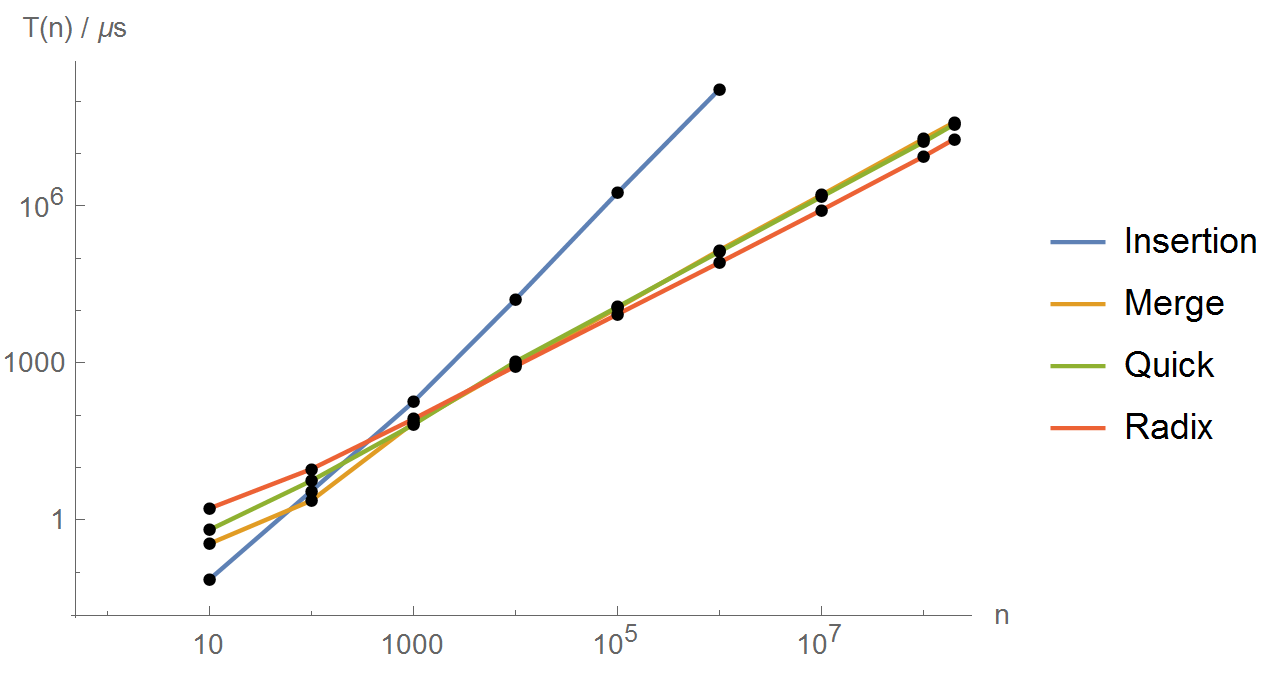
\includegraphics[width=0.75\columnwidth]{chart}
\end{center}

It's clear that insertion sort has the greatest time complexity $\Theta(n^2)$, while radix sort has the least $\Theta(n)$.

Quick sort and merge sort are in between, and are basically the same on random arrays. As size of the array grows, quick sort has the shorter running time.
}
\end{homeworkProblem}


%----------------------------------------------------------------------------------------

\end{document}
